\stepcounter{appendixnum}
\renewcommand{\thechapter}{\Asbuk{appendixnum}}
\chapter{{\fontsize{14pt}{21pt}\selectfont\MakeUppercase{ПРИЛОЖЕНИЕ \appendixletter}}}
\label{cha:appendix3}

\setcounter{figure}{0}
\renewcommand{\thefigure}{\appendixletter.\arabic{figure}}

\begin{figure}[H]
\centering
\begin{mdframed}
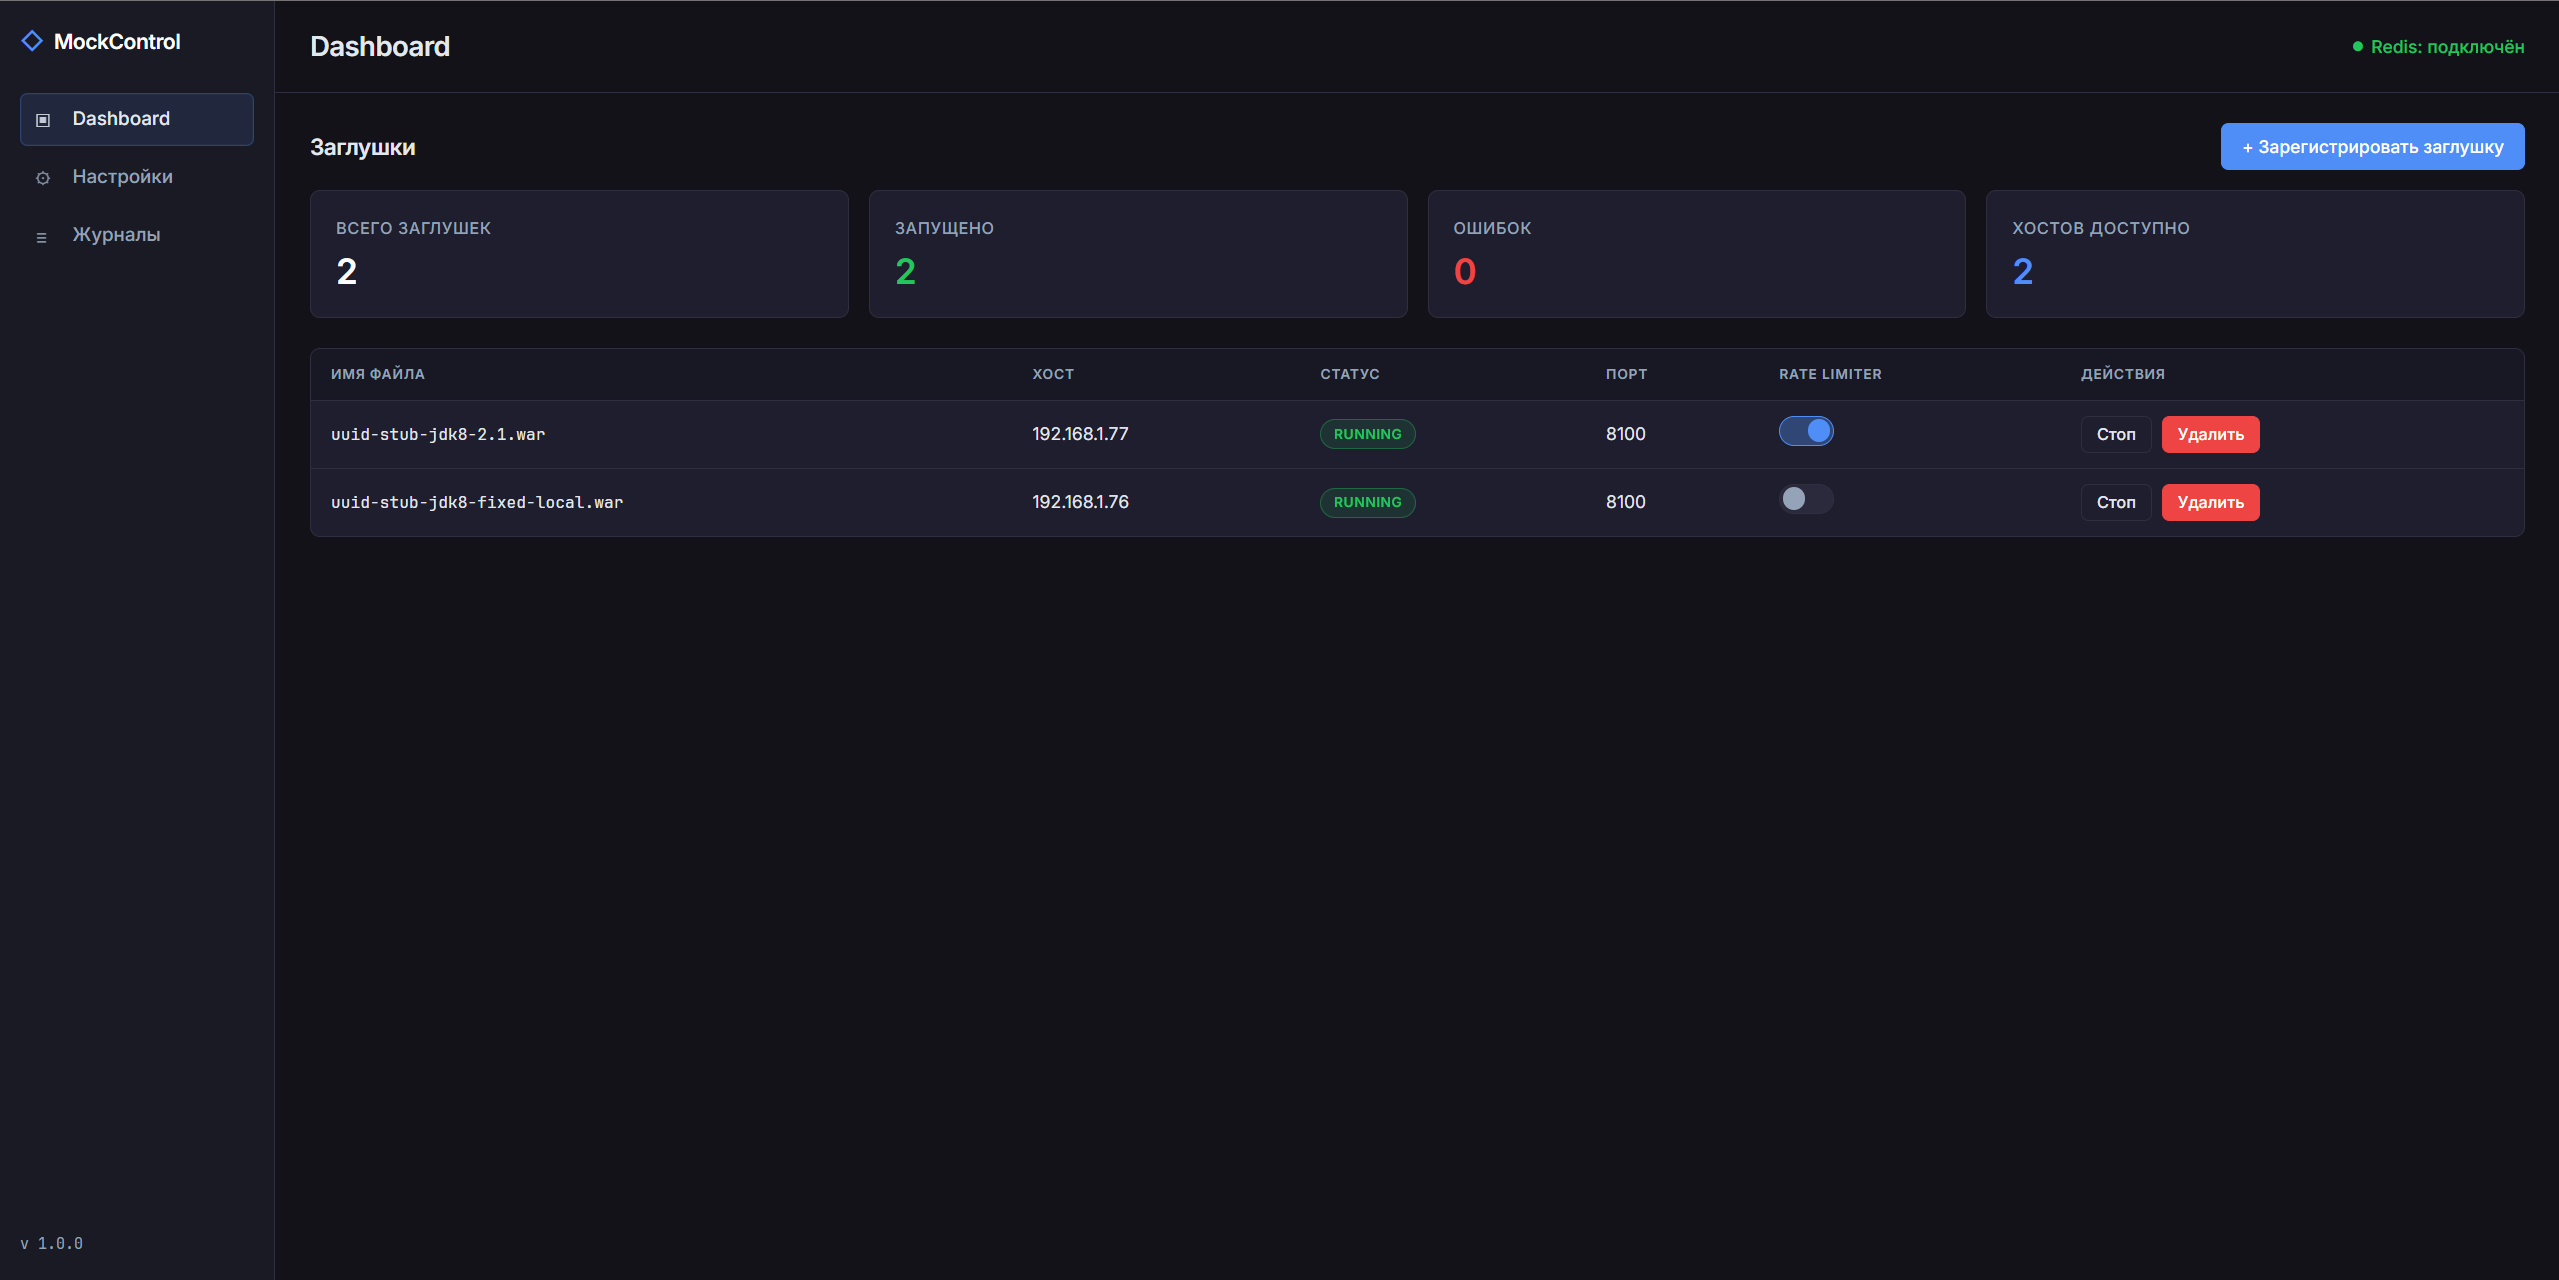
\includegraphics[width=\textwidth]{images/impl-dashboard.png}
\end{mdframed}
\caption{Реализованная главная панель управления}
\label{fig:impl-dashboard}
\end{figure}

\begin{figure}[H]
\centering
\begin{mdframed}
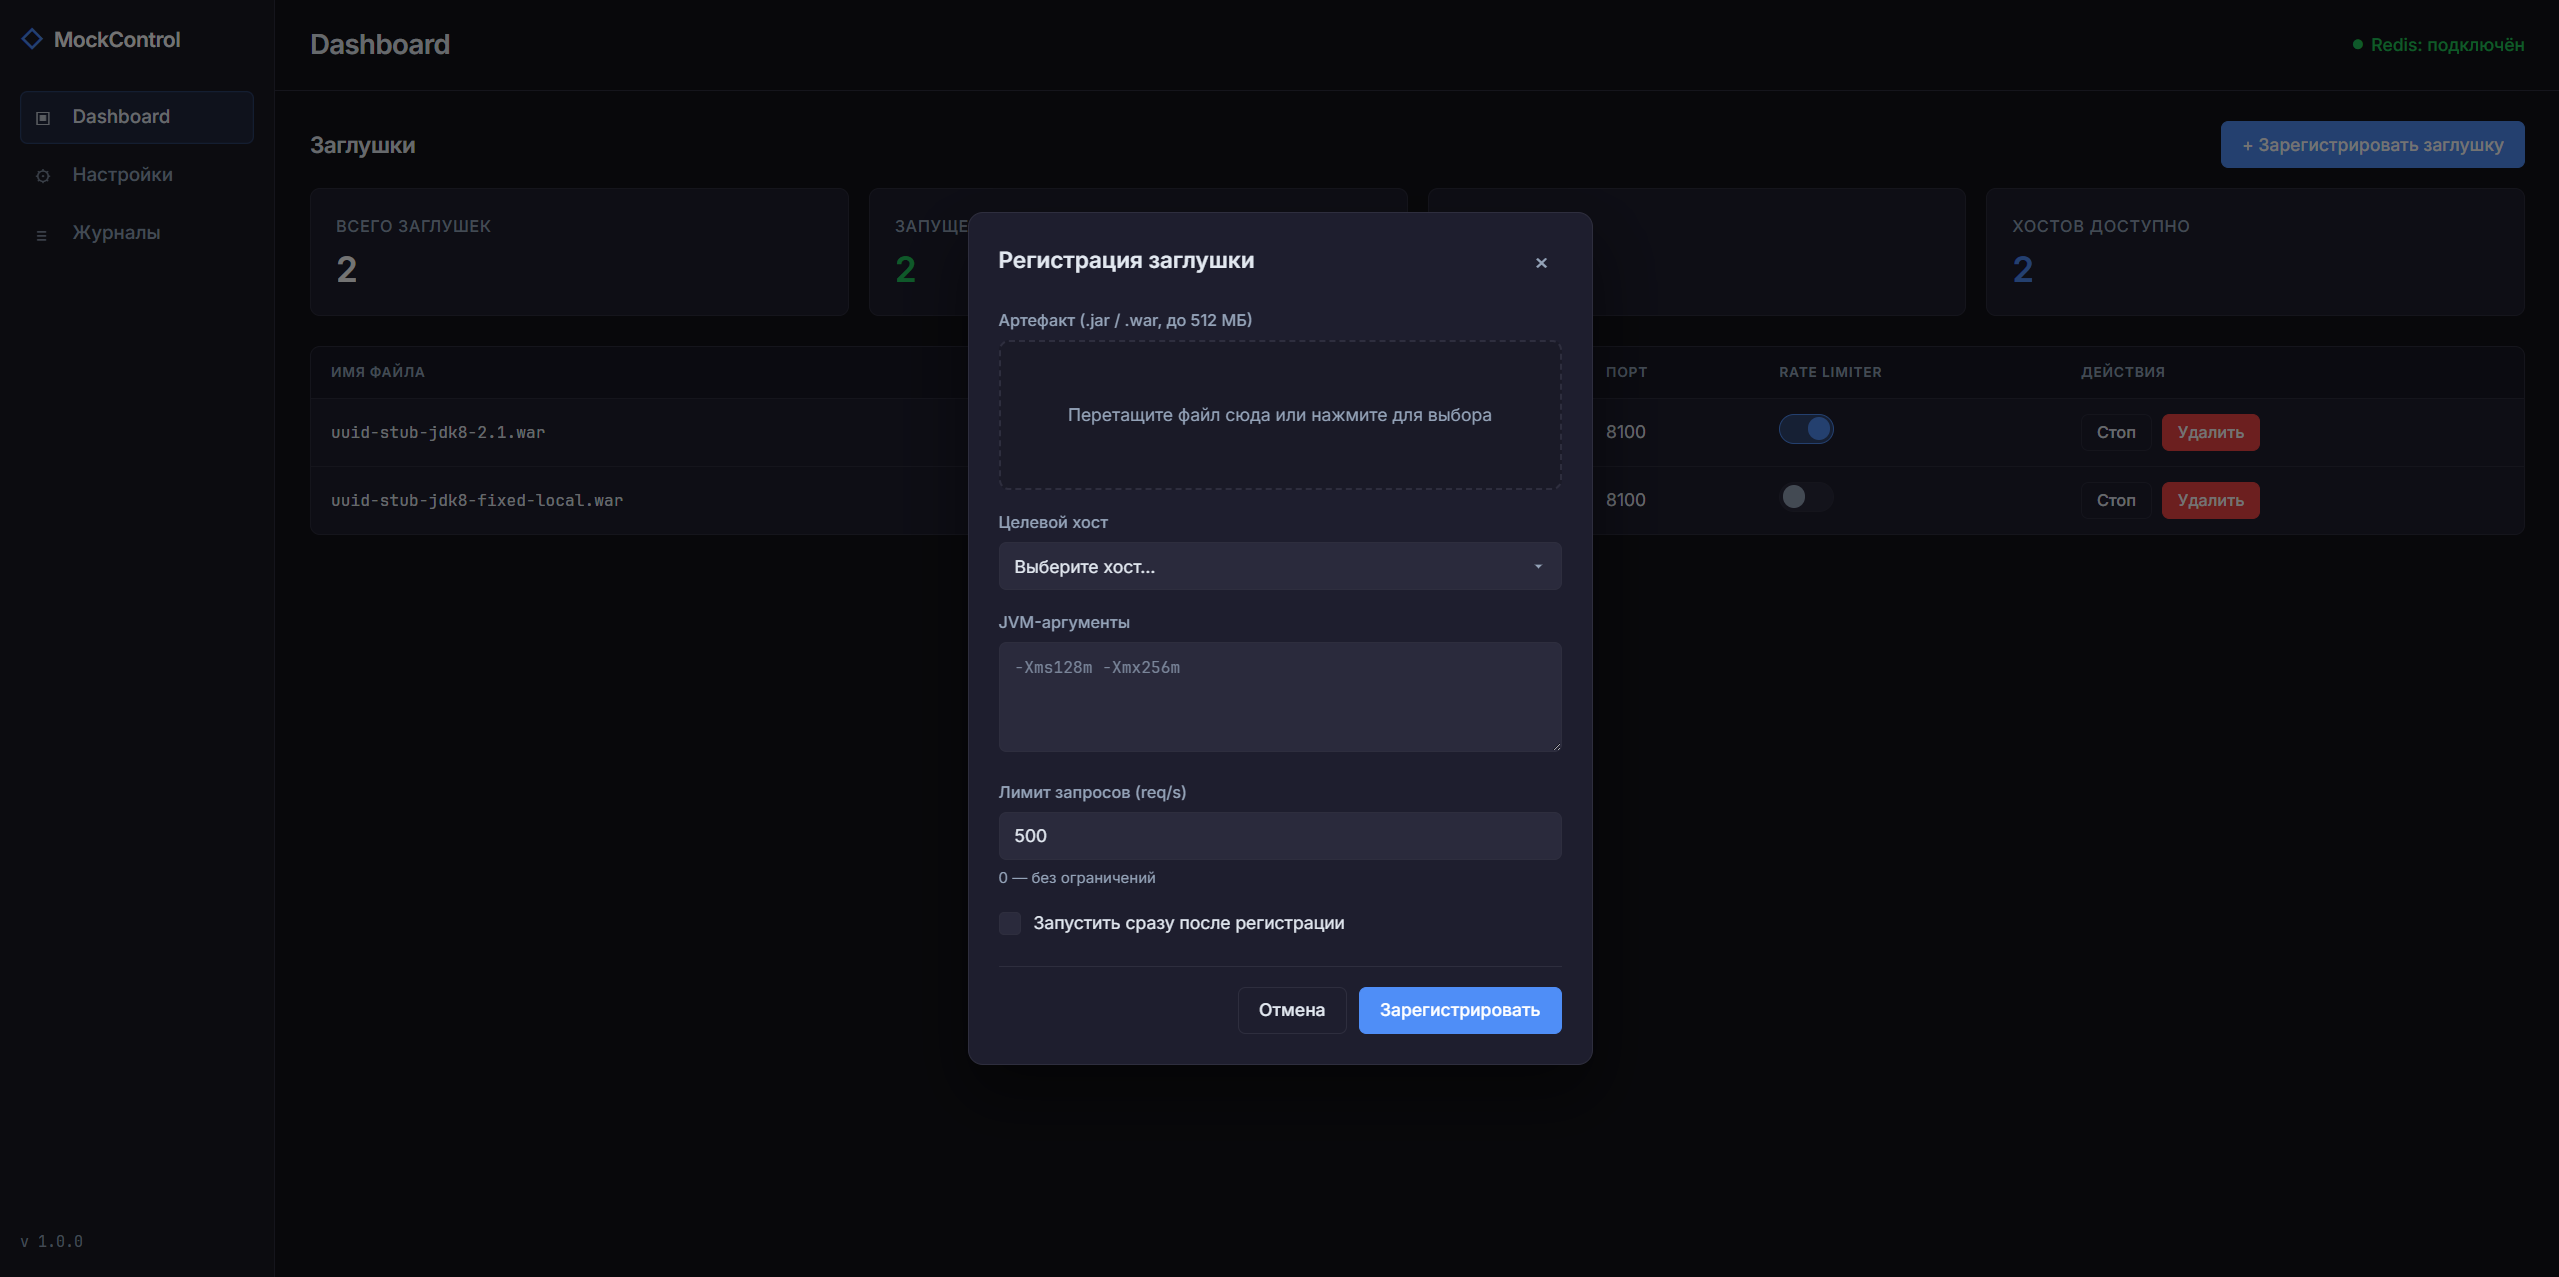
\includegraphics[width=\textwidth]{images/impl-register-modal.png}
\end{mdframed}
\caption{Реализованное диалоговое окно регистрации заглушки}
\label{fig:impl-register-modal}
\end{figure}

\begin{figure}[H]
\centering
\begin{mdframed}
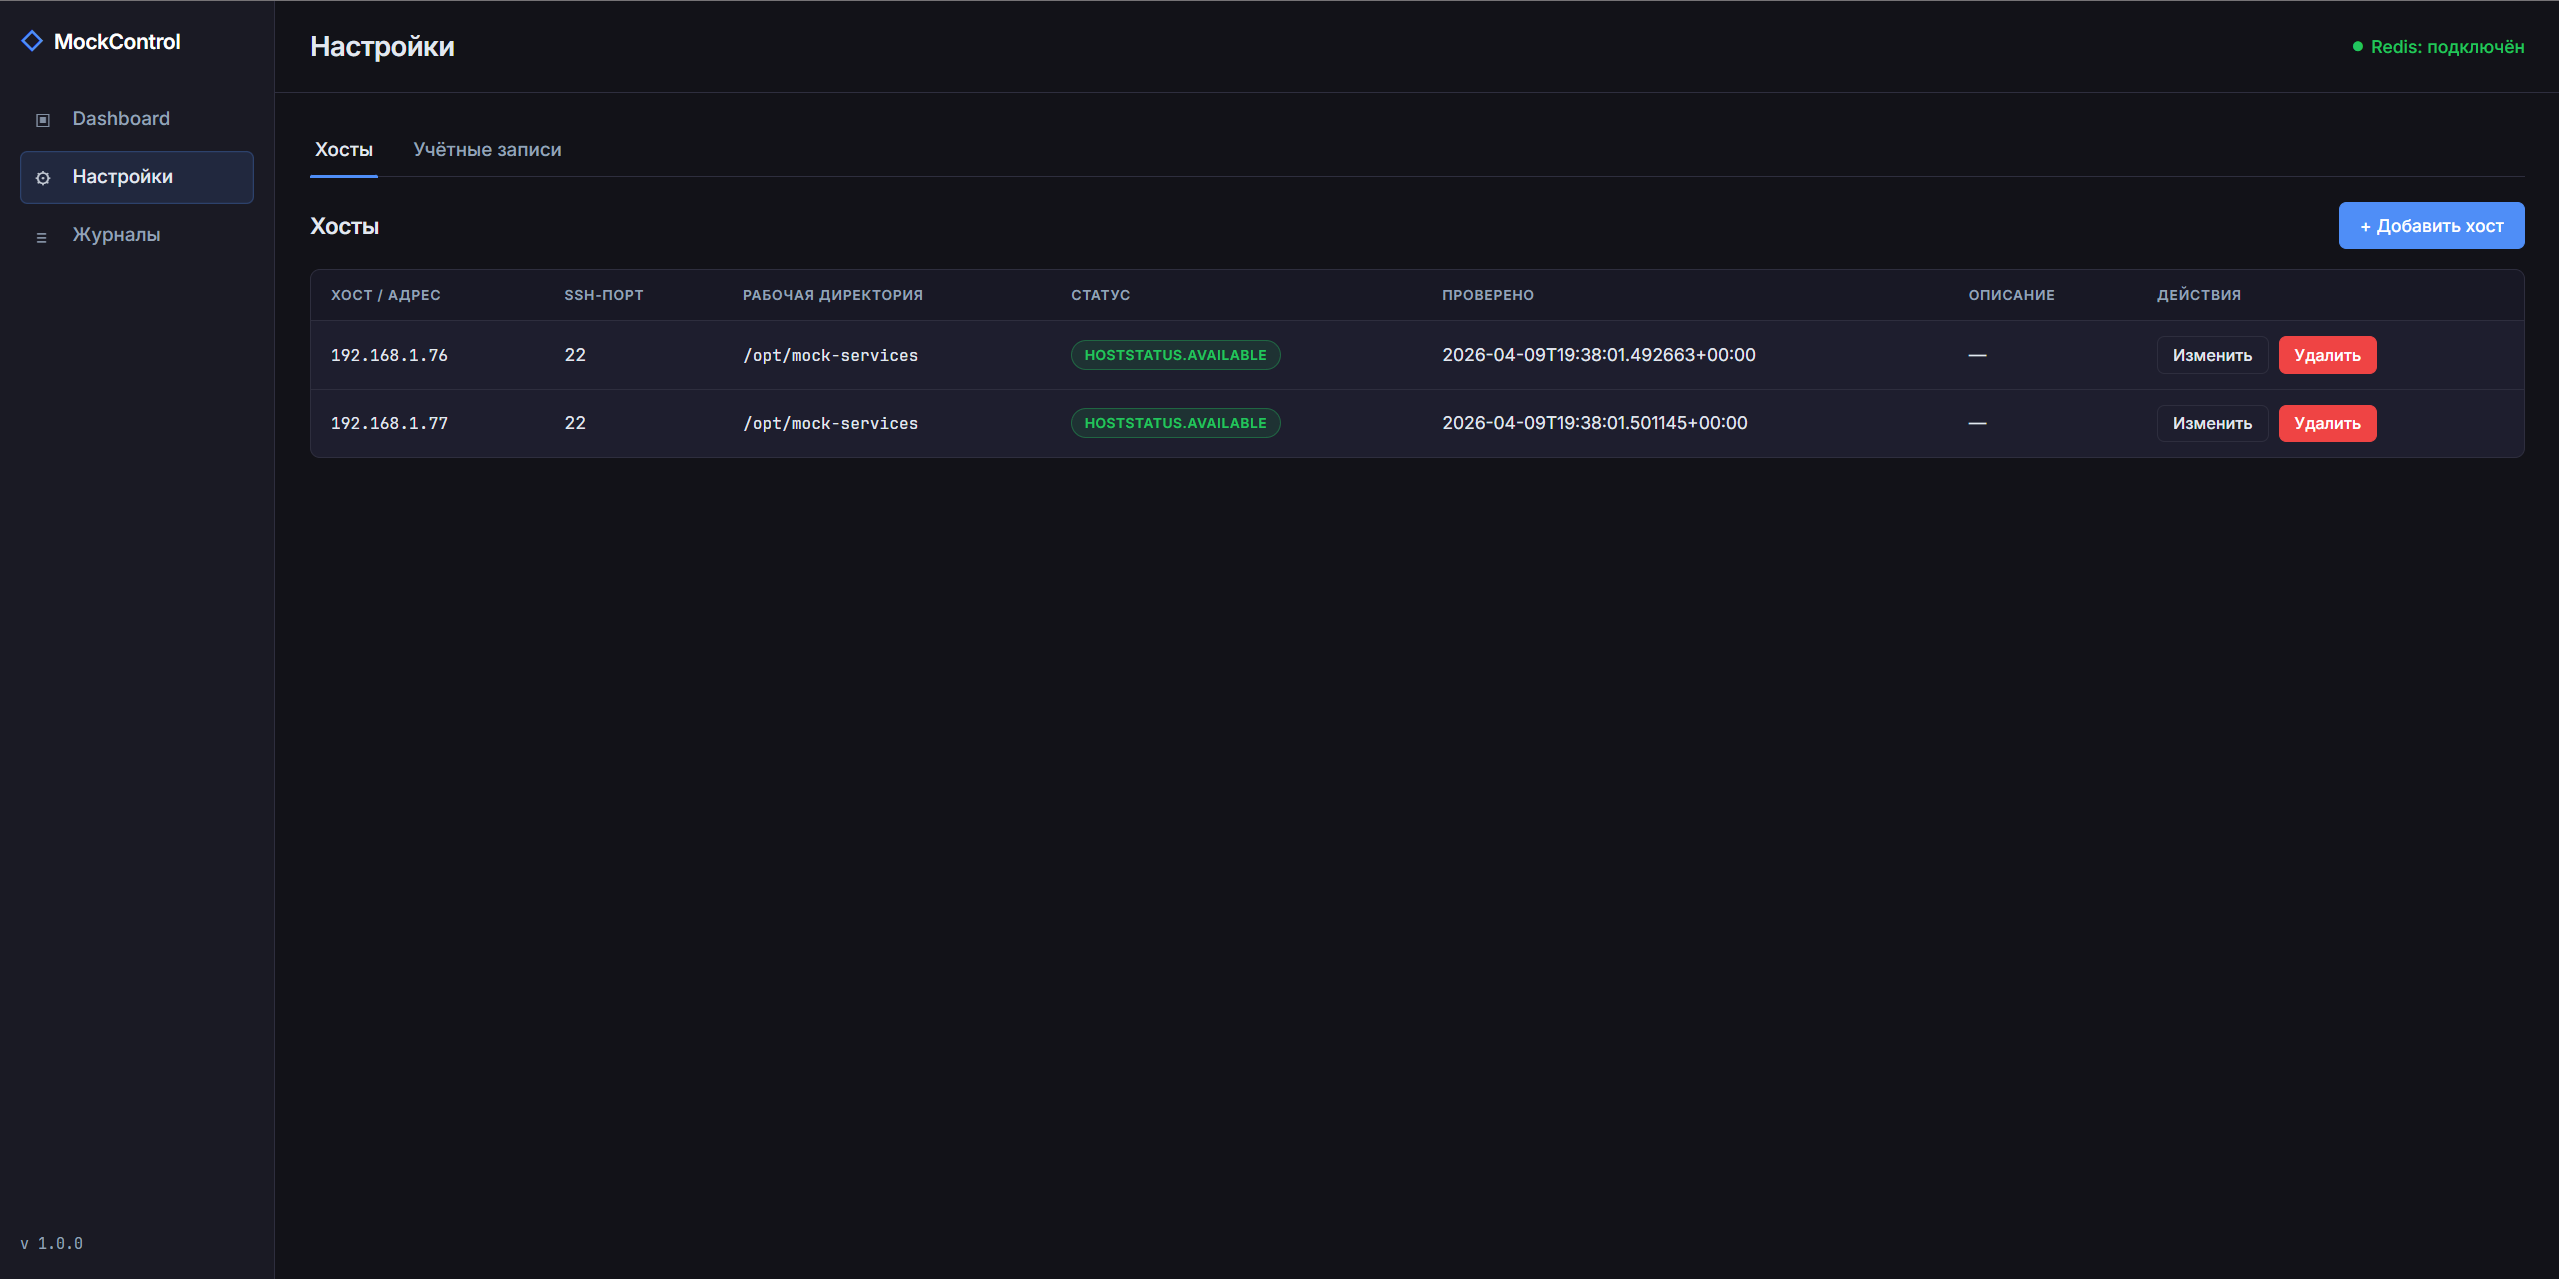
\includegraphics[width=\textwidth]{images/impl-settings-hosts.png}
\end{mdframed}
\caption{Реализованная страница настроек, вкладка «Хосты»}
\label{fig:impl-settings-hosts}
\end{figure}

\begin{figure}[H]
\centering
\begin{mdframed}
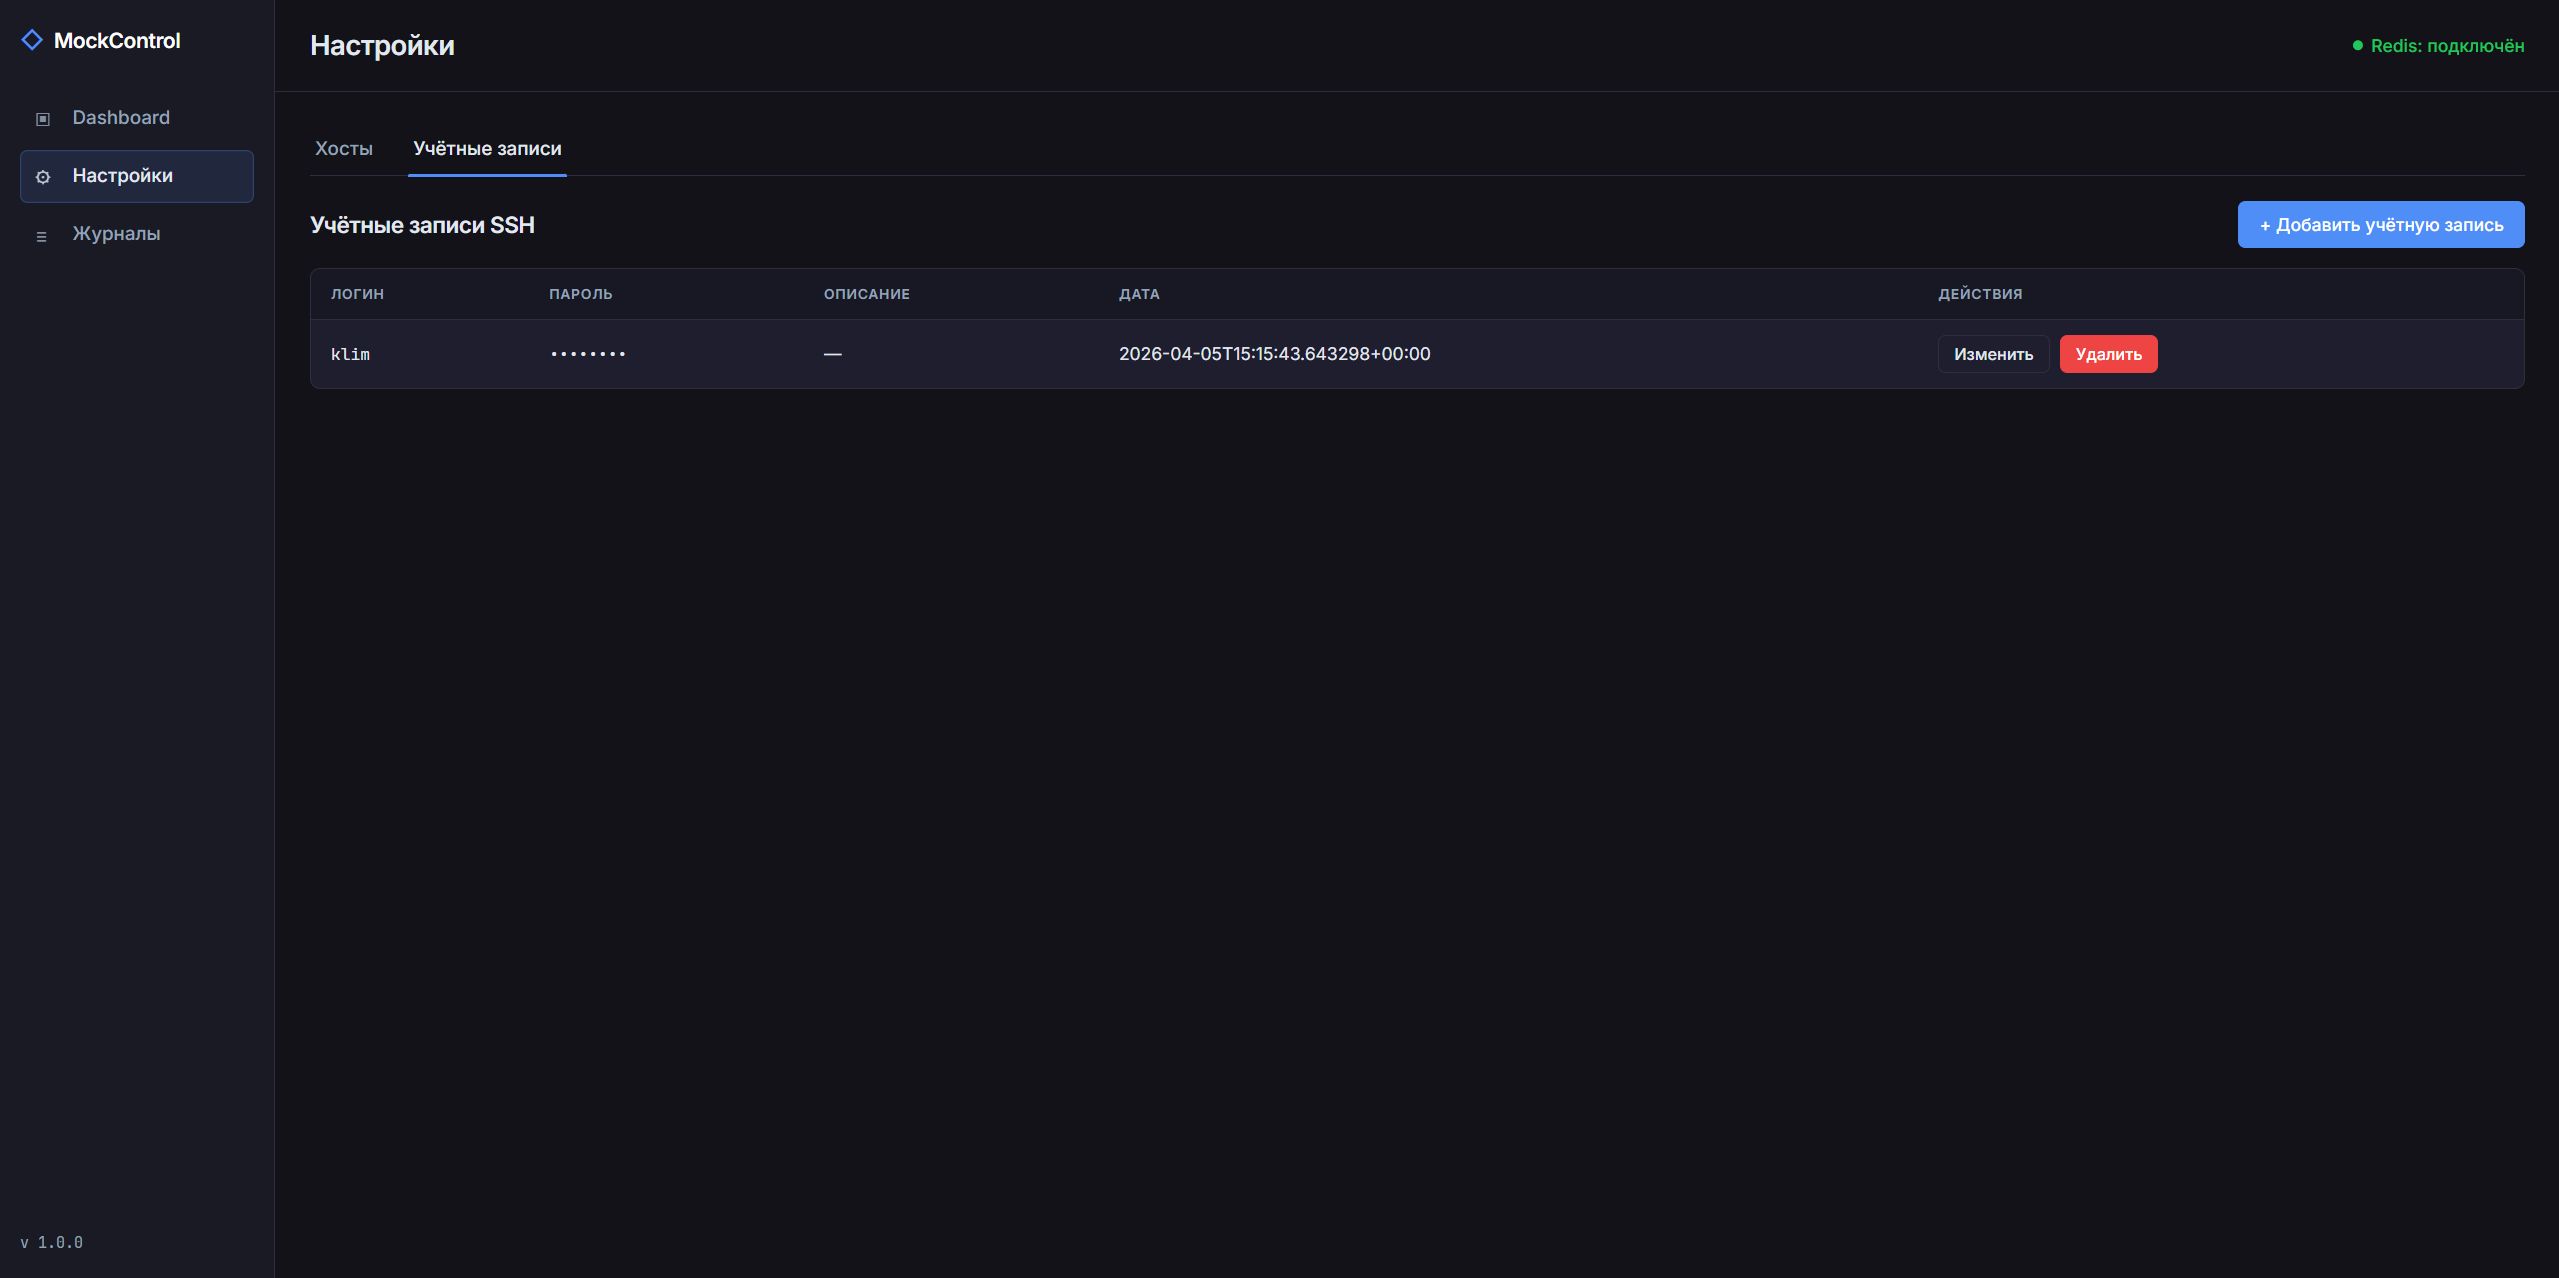
\includegraphics[width=\textwidth]{images/impl-settings-accounts.png}
\end{mdframed}
\caption{Реализованная страница настроек, вкладка «Учётные записи»}
\label{fig:impl-settings-accounts}
\end{figure}

\begin{figure}[H]
\centering
\begin{mdframed}
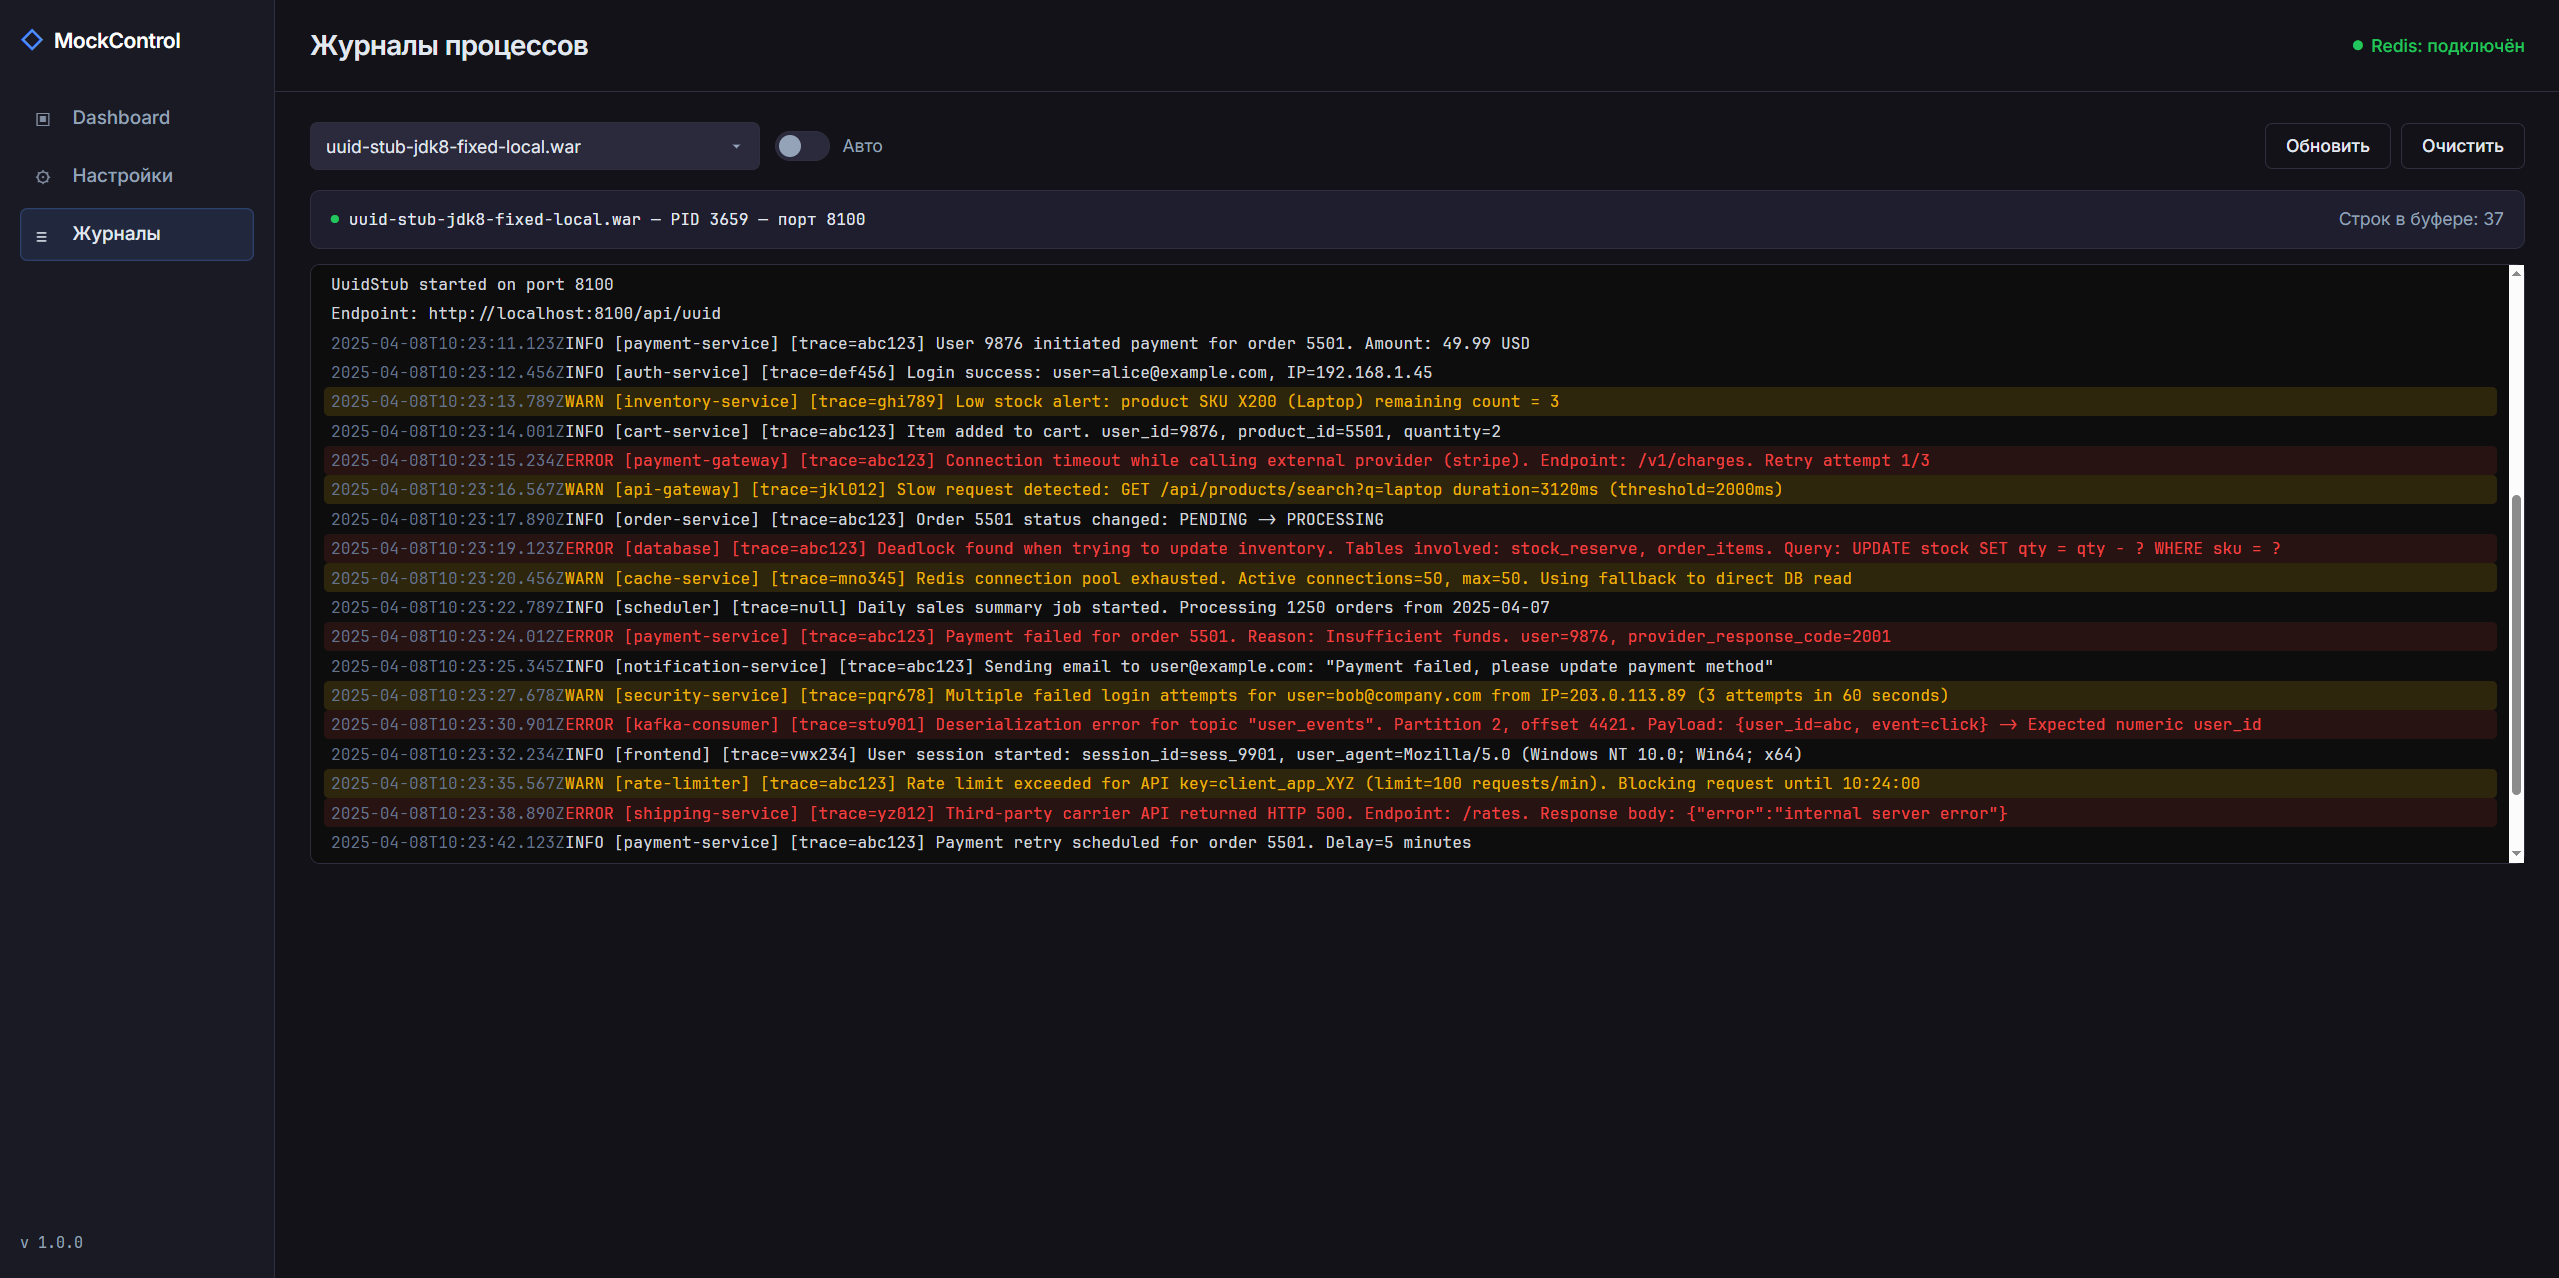
\includegraphics[width=\textwidth]{images/impl-logs.png}
\end{mdframed}
\caption{Реализованная страница просмотра журналов процессов}
\label{fig:impl-logs}
\end{figure}
